\section{Schlussfolgerungen}
Die Untersuchungen haben aufgezeigt, dass die Klasse der evolutionären Algorithmen zum finden von endlichen Automaten zu gegebenen regulären Ausdrücken folgende Eigenschaften aufweisen:
\begin{itemize}
	\item Verfahren mit einer konstanten Problemmenge skalieren stark mit der Grösse ebendieser
	\item Alle Verfahren skalieren mit der Anzahl Lösungskandidaten
	\item Globale Selektionsverfahren konvergieren schneller als lokale
\end{itemize}

\subsection{Skalierung mit der Problemmengengrösse}
Die Skalierung mit der Problemmengengrösse erschloss sich mir nach einem Brainstorming zum Thema Mengenlehre.

\begin{figure}[h]
  \centering
  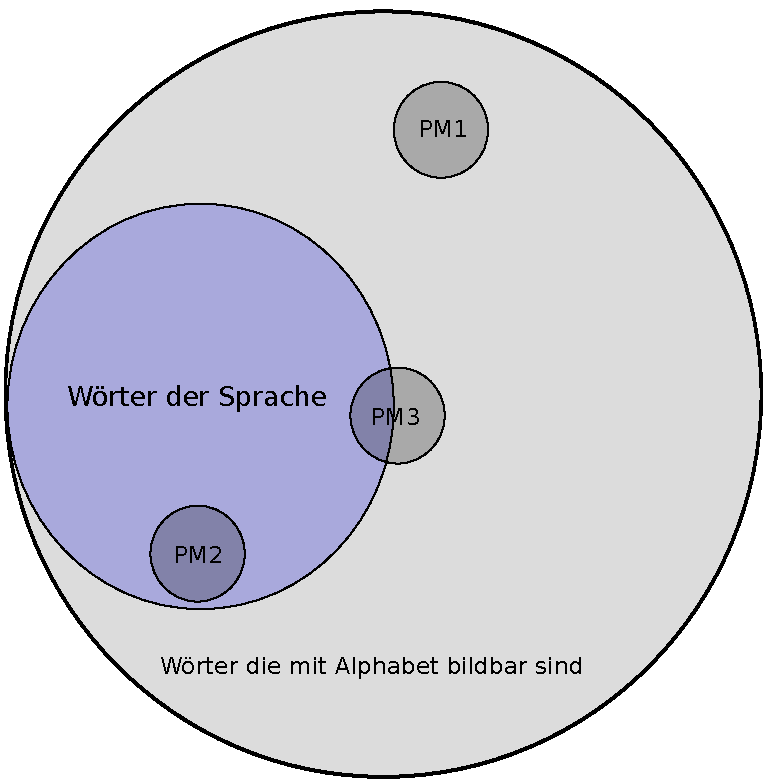
\includegraphics[width=0.4\textwidth]{images/problemmengen.pdf}
  \caption[Problemmengen]{Problemmengen}
  \label{fig:problemmengen}
\end{figure}

In Abbildung \ref{fig:problemmengen} sind die (unendliche) Menge aller bildbaren Wörter mit dem gegebenen Alphabet, die (bei unseren Beispielen ebenfalls unendliche) Menge aller Wörter der entsprechenden Sprache (bei uns repräsentiert durch reguläre Ausdrücke und endliche Automaten) und mögliche Problemmengen (PM1 bis PM3) abgebildet.
\begin{itemize}
	\item PM1: Diese Problemmenge beinhaltet kein einziges Wort der Sprache. Damit lässt sich nicht testen ob ein Automat Wörter der Sprache erkennt.
	\item PM2: Diese Problemmenge beinhaltet nur Wörter der Sprache. Damit lässt sich nicht testen ob ein Automat Wörter die nicht in der Sprache sind nicht akzeptiert.
	\item PM3: Diese Problemmenge beinhaltet sowohl Wörter der Sprache als auch solche die nicht zur Sprache gehören. Eine solche Problemmenge wäre die Voraussetzung wenn ein Algorithmus konvergieren soll.
\end{itemize}

Die Wahrscheinlichkeit eine Problemmenge mit den Eigenschaften von PM3 zu erhalten hängt sowohl von der Menge der generierten Probleme, als auch vom Verhältnis der Menge aller bildbaren Wörter zur Menge aller Wörter der Sprache ab. Ersteres erklärt warum mutierenden Problemmengen mit kleineren Problemmengen auskommen. Sie generieren nach jedem Zyklus $\frac{p}{2}$ (wenn $p$ die Grösse der Problemmenge ist) neue Probleme und generieren so in ihrere Laufzeit viel mehr Probleme als ihre konstanten Gegenstücke. Letzteres erklärt warum die Algorithmen mit den unterschiedlichen Problemstellungen unterschiedlich oft konvergieren. Bei den beiden Binärzahlen-Teilbarkeitsproblemen ist das Verhältnis aller Binärwörter zum Verhältnis der Wörter der 1:3 bzw. 1:5. Beim ABAB Problem ist dieses Verhältnis bedeutend kleiner (rund 1:16).

\subsection{Skalierung mit der Anzahl Lösungskandidaten}
Die Skalierung mit der Anzahl Lösungskandidaten lässt sich dadurch erklären, dass der Algorithmus nur konvergieren kann wenn ein genügend grosses Gefälle in der Fitnessverteilung vorhanden ist.

\begin{figure}[h]
  \centering
  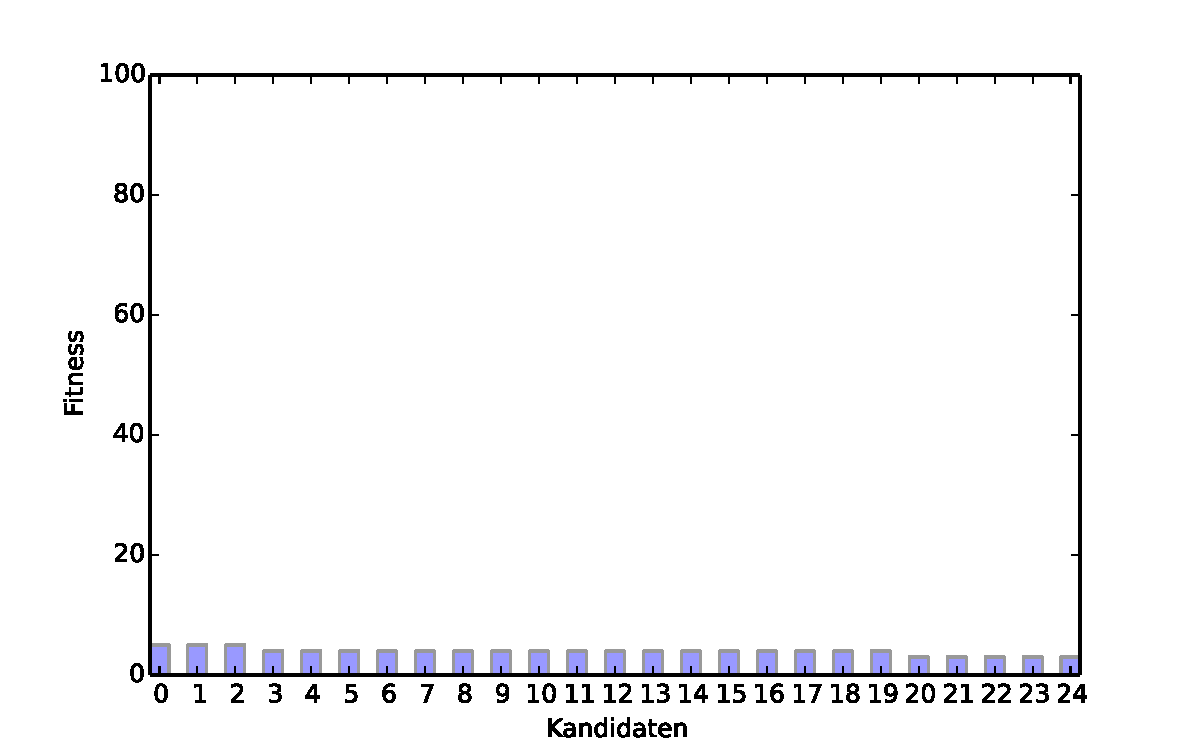
\includegraphics[width=0.7\textwidth]{images/bars_fitness.pdf}
  \caption[Zu geringes Gefälle in der Fitnessverteilung]{Zu geringes Gefälle in der Fitnessverteilung}
  \label{fig:bars_fitness.pdf}
\end{figure}

In der Abbildung \ref{fig:bars_fitness.pdf} ist ersichtlich, dass in diesem Beispiel alle Kandidaten schlecht (circa. $5$ bei $\max 100$) konditioniert sind und dass praktisch kein Gefälle vorhanden ist. Dies kann verschiedene Ursachen haben:

\begin{itemize}
	\item Es wurden zufällig einfach sehr ähnliche oder zumindest ähnlich schlecht konditionierte Automaten generiert 
	\item Die verwendete Problemmenge beinhaltet nur oder gar keine Wörter der Sprache
	\item Die verwendete Problemmenge ist zu klein
\end{itemize}

Die Wahrscheinlichkeit, dass Ersteres eintritt wird durch das verwenden von mehr Lösungskandidaten vermindert. Die anderen beiden Faktoren müssen über die Problemmenge abgefangen werden. Das verwenden von mehr Lösungskandidaten führt auch in jedem Falle dazu, dass die Wahrscheinlichkeit bereits bei der Initialisierung einen oder mehrere sehr gute Automaten zu generieren steigt. Die Kehrseite des Ganzen ist, dass der Rechenaufwand linear mit der Anzahl Lösungskandidaten steigt. 

\subsection{Lokale vs. globale Selektionsverfahren}
Warum lokale Selektionsverfahren weniger schnell konvergieren als globale zeigte sich nach dem plotten von Fitnesswerten und dem entsprechenden Evolutionsverhalten.

\begin{figure}[h]
  \centering
  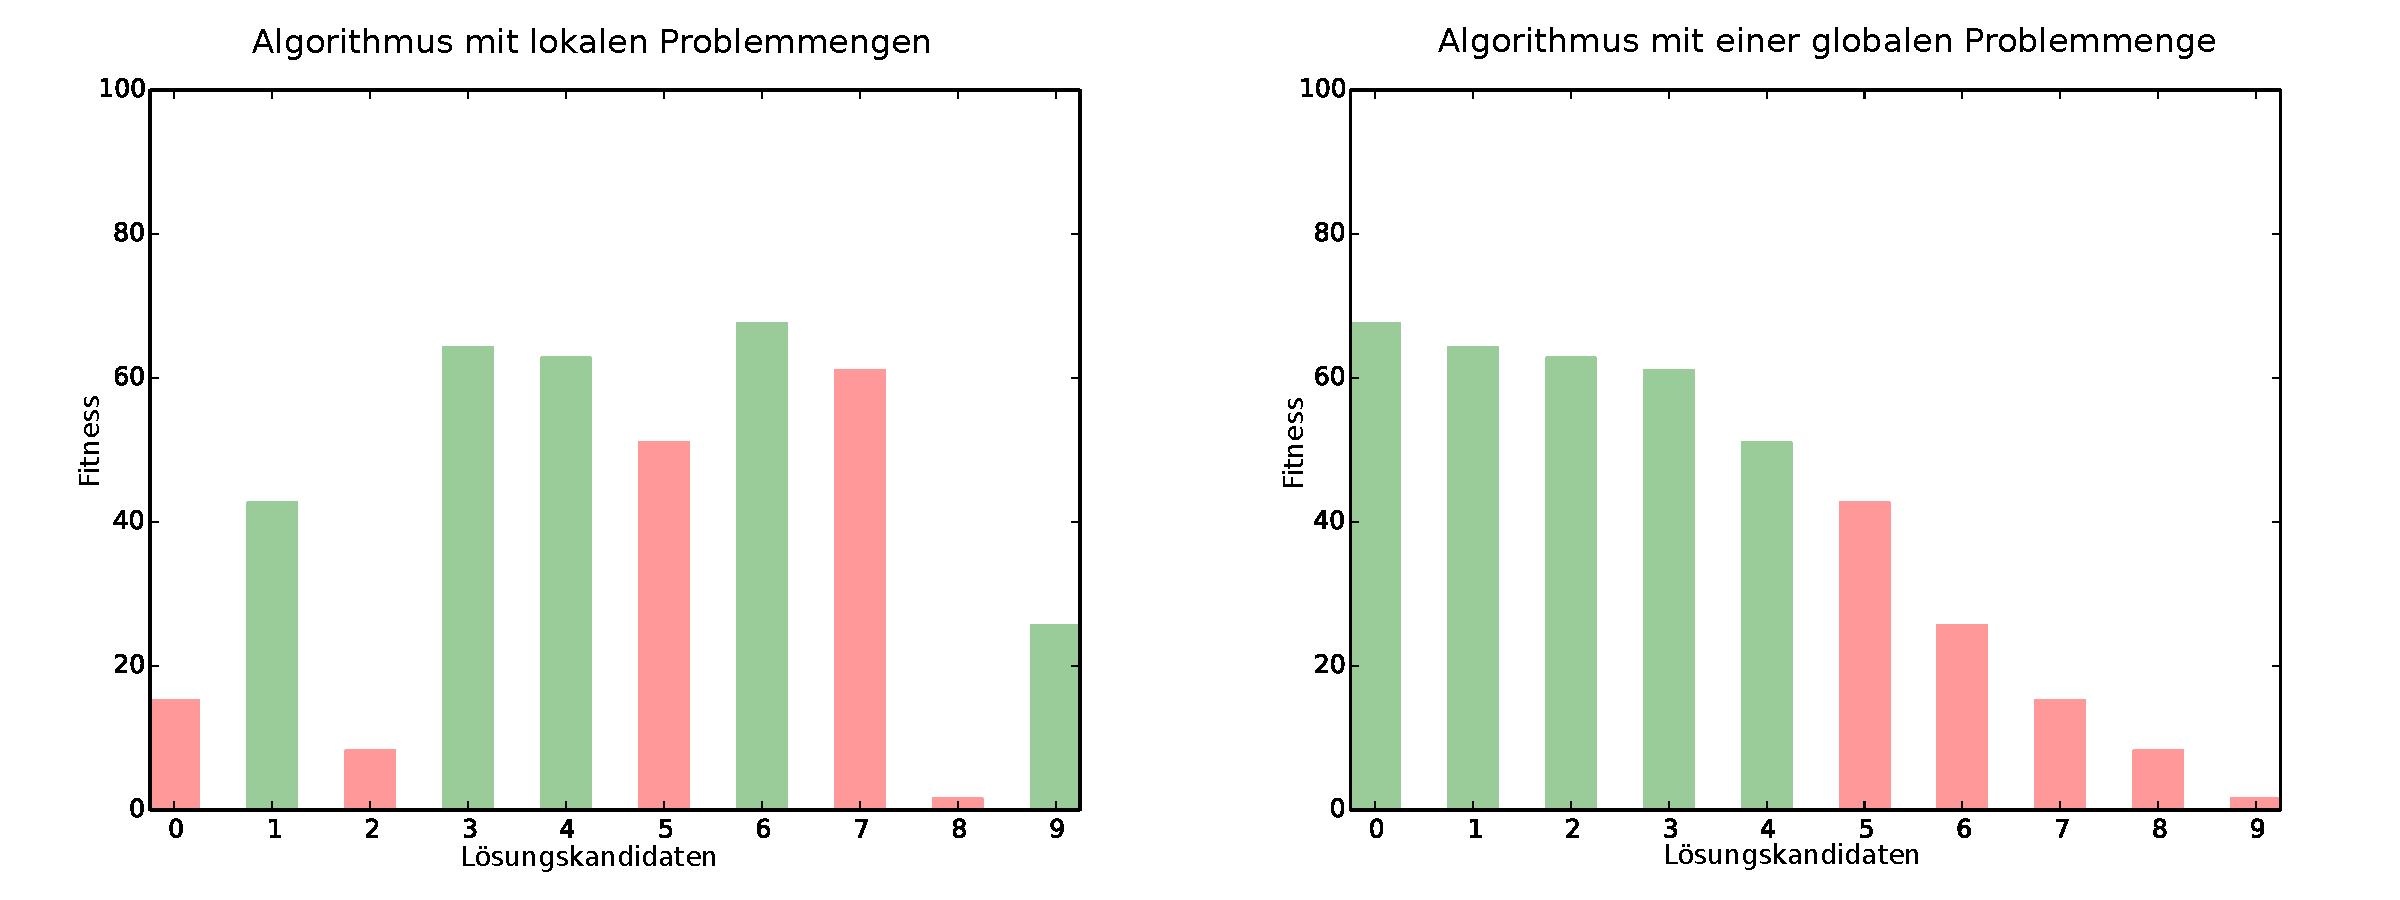
\includegraphics[width=0.8\textwidth]{images/evolutionsverhalten_lokal_vs_global.pdf}
  \caption[Evolutionsverhalten lokale Problemenge vs. globale Problemmenge]{Evolutionsverhalten lokale Problemenge vs. globale Problemmenge}
  \label{fig:evolutionsverhalten_lokal_vs_global}
\end{figure}

In der Abbildung \ref{fig:evolutionsverhalten_lokal_vs_global} sind links und rechts die selben Lösungskandidaten abgebildet. Grün eingefärbt sind diejenigen, welche die nächste Runde erreichen, rot die aussterbenden. In der linken Grafik sterben die Lösungskandidaten 5 und 7 aus obwohl sie besser sind als die Kandidaten 1 und 9. Dies ist so, weil für dieses Verfahren ein \flqq 1 vs. 1\frqq Selektionsverfahren implementiert wurde (Siehe Kapitel \ref{subsec:LocalEvolvingProblemSet}). Das heisst, dass hier jeweils die Lösungskandidaten 0 und 1, 2 und 3, 4 und 5 etc. gegeneinander antreten und der jeweils bessere weiter kommt. Wie gut die Automaten im Vergleich zum grossen Ganzen sind ist irrelevant.